% !TEX output_directory = ./.temp/report
% !TEX options = --shell-escape

\documentclass[a4paper, 12pt]{scrartcl}
\usepackage[assign-num=3]{report}
\usepackage[outputdir=./.temp/report]{minted}

\title{Comparison of Game Engines}

\begin{document}

\maketitle

\section{Introduction}
A game engine is a tool for developers of video games. It is software framework which abstracts away core parts of a video game such as rendering, physics, input handling, sound, AI, etc. It typically includes software libraries and other software in the form of a software development kit (SDK), which contains additional tools revolving around the engine's ecosystem (level editor, asset packager, and so on).

A game engine enables developers to create games more efficiently, since a lot of the fundamental components of a game are available for use out of the box. This saves developers the time of having to implement all these core features from scratch, which could otherwise add a tremendous amount of complexity to the project. For example, game engines may offer cross-platform capabilities in a more or less transparent way to the developers. This removes the necessity to deal with the plethora of different platform-specific APIs, which allows developers and publishers to reach a broader market more easily.

\subsection{History}
Game engines were not immediately prevalent in the industry when it first started. This is because the platforms were much more fragmented, and there was little standardisation (and thus little compatibility) among them. Furthermore, hardware was being developed at a rapid pace. All these factors made it difficult to re-use any abstractions (such as those provided by a game engine) in the long term. Hardware was also quite limited, so it was necessary to build a game's components from scratch and custom-tailor them to the target platform to ensure the game ran optimally.

The earliest software that may constitute a game engine was in-house for use with first-party software. These engines were far more limited in scope than modern game engines (what may now be considered \textit{middleware} used by a game engine). Engines for third-parties became prevalent in the 1990s along with the growing popularity and feasibility of 3D graphics. This led to influential engines such as id Tech and Unreal Engine, which are in some form or another still in use with modern games.

Such engines were developed for first-party games, but made available for licensing to third-party developers. Companies shifted their strategy to developing the game and its engine separately. This decoupling enabled the engine to be usable by third parties, and allowed developers to become more specialised.

\section{Comparing Source and Unity}
This section compares and contrasts various aspects of two different engines: Source by Valve Software and Unity by Unity Technologies.

\subsection{Development Environment}
\subsubsection{Source}
Programming is done in C++, typically using Visual Studio. However, other IDEs can also work. A level editor named \textit{Hammer} is included in the Source SDK. When not programming or making assets, this is tool that is being worked with the most. It is used to define the level's geometry, apply textures, light the level, place objects and entities, configure behaviour logic for entities, and much more.

\begin{figure}[!htp]
  \centering
  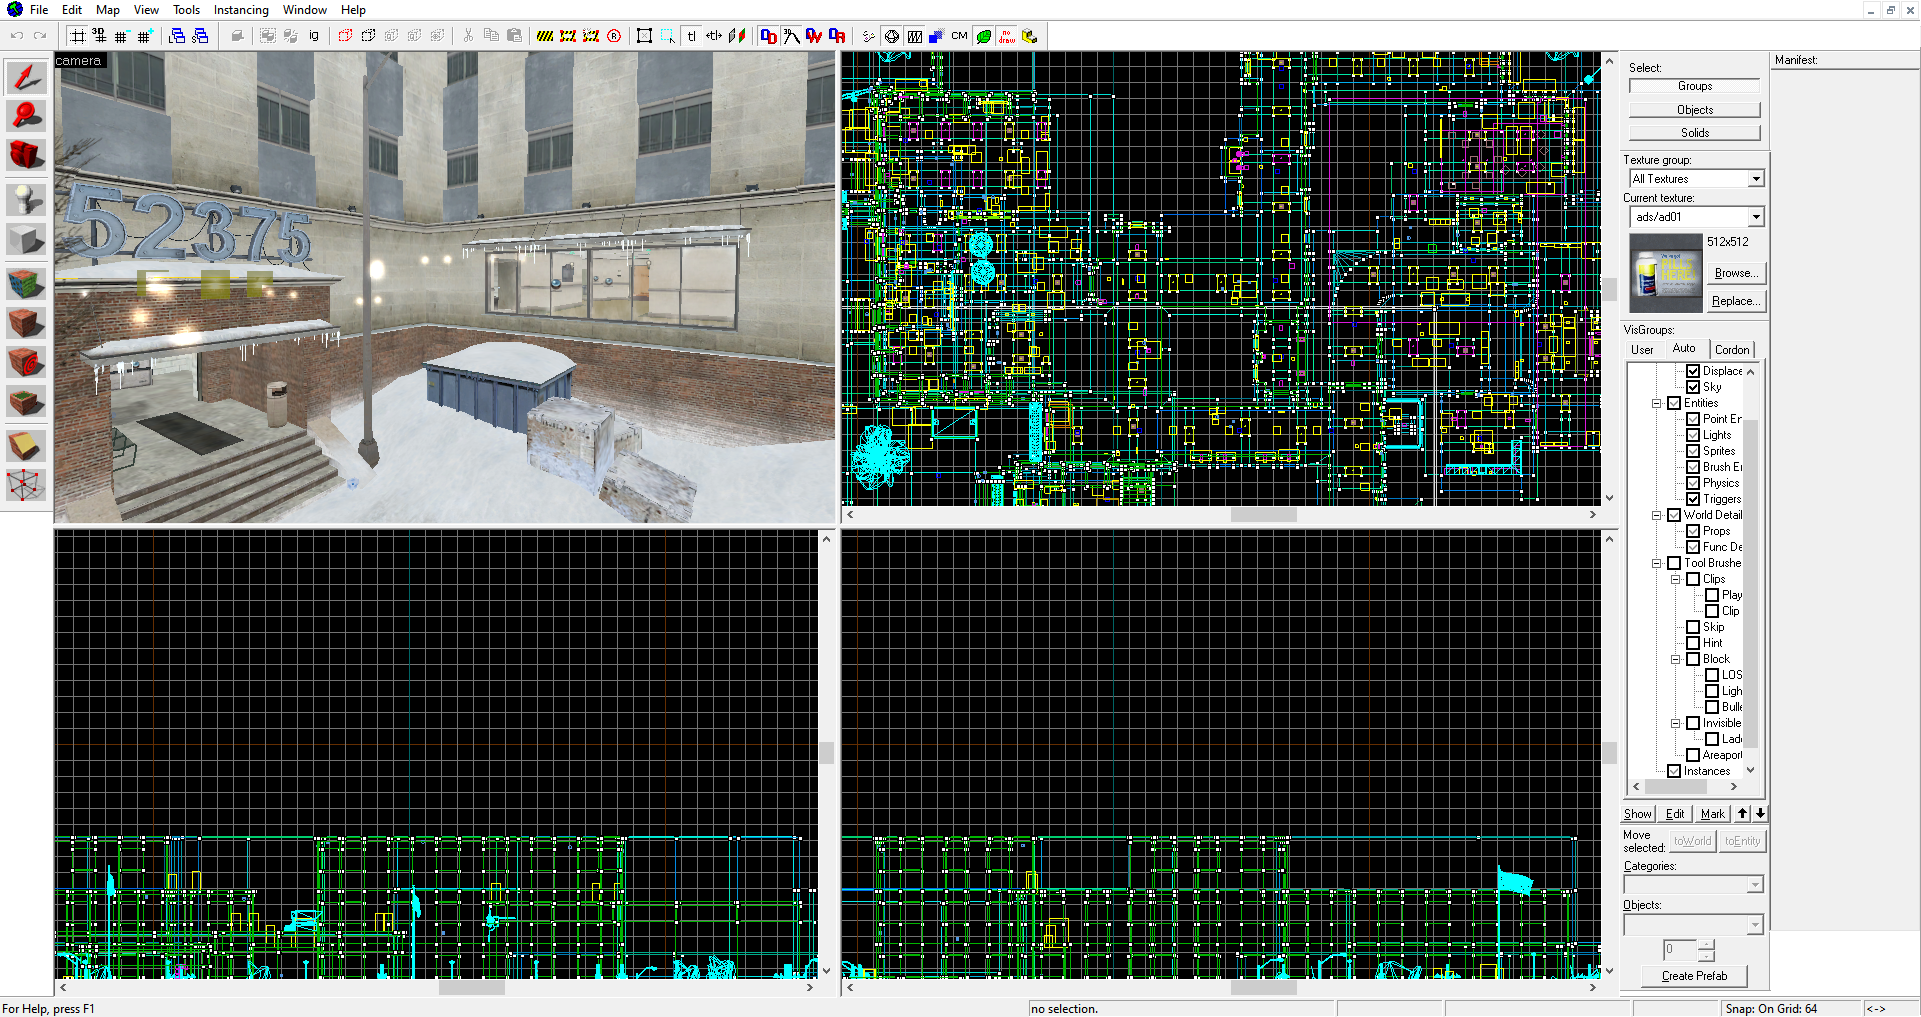
\includegraphics[width=\linewidth]{images/source_hammer.png}
  \caption{Hammer editing \textit{cs\_office} from CS:GO}
\end{figure}

Assets such as models and textures are expected to be created using third-party tools. For modelling, Autodesk XSI and Maya were historically popular. However, it's more common these days to use one of the third-party plugins for other modelling tools such as Blender.

Some assets, including models and textures, are expected to be in Source-specific formats. To achieve this, the Source SDK provides some command-line tools to convert assets to the expected formats. For example, \texttt{vtex} is used for texture conversion and \texttt{studiomdl} is used to compile models. There are various other command-line tools, like \texttt{vbsp}, \texttt{vvis}, and \texttt{vrad} for map compilation and \texttt{vpk} for packaging game assets.

There are also third-party tools frequently used by modders and level designers, such as VIDE, which can be used to create textures, view or create game content packages, edit particles, pack game content into map files, and much more.

\begin{figure}[!htp]
  \centering
  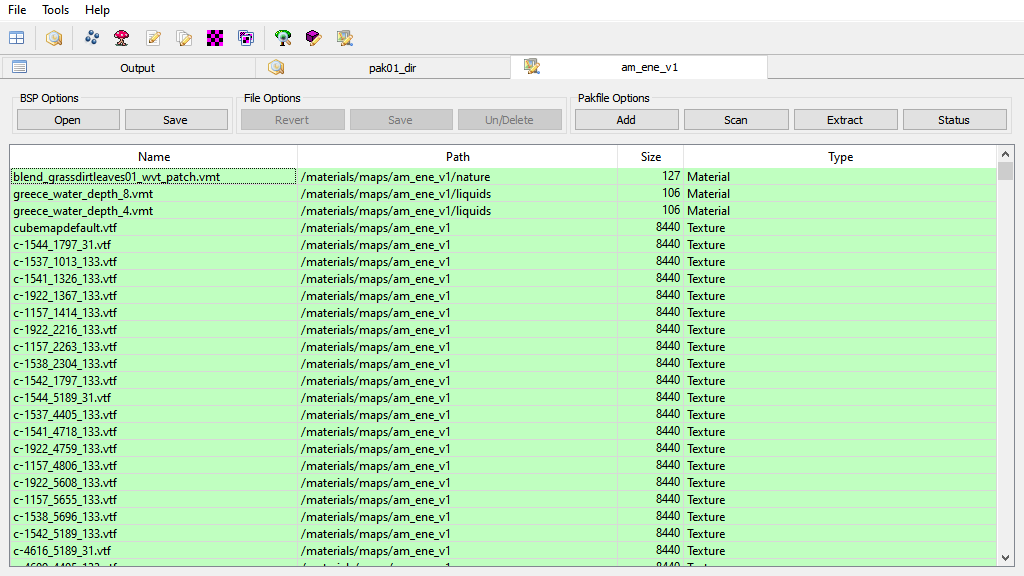
\includegraphics[width=\linewidth]{images/source_vide_pakfile.png}
  \caption{VIDE displaying the pakfile lump of a map}
\end{figure}

\subsubsection{Unity}
The primary development environment for Unity is the Unity Editor. This environment is quite integrated; the Source engine's environment looks dated and fragmented in comparison. Like Hammer, Unity Editor can define the geometry of a scene and apply textures to objects. But it could also do a lot more, like creating animations and materials, running the game within, inspecting a running game's state, designing UIs, creating visual effects, and profiling the game.

\begin{figure}[!htp]
  \centering
  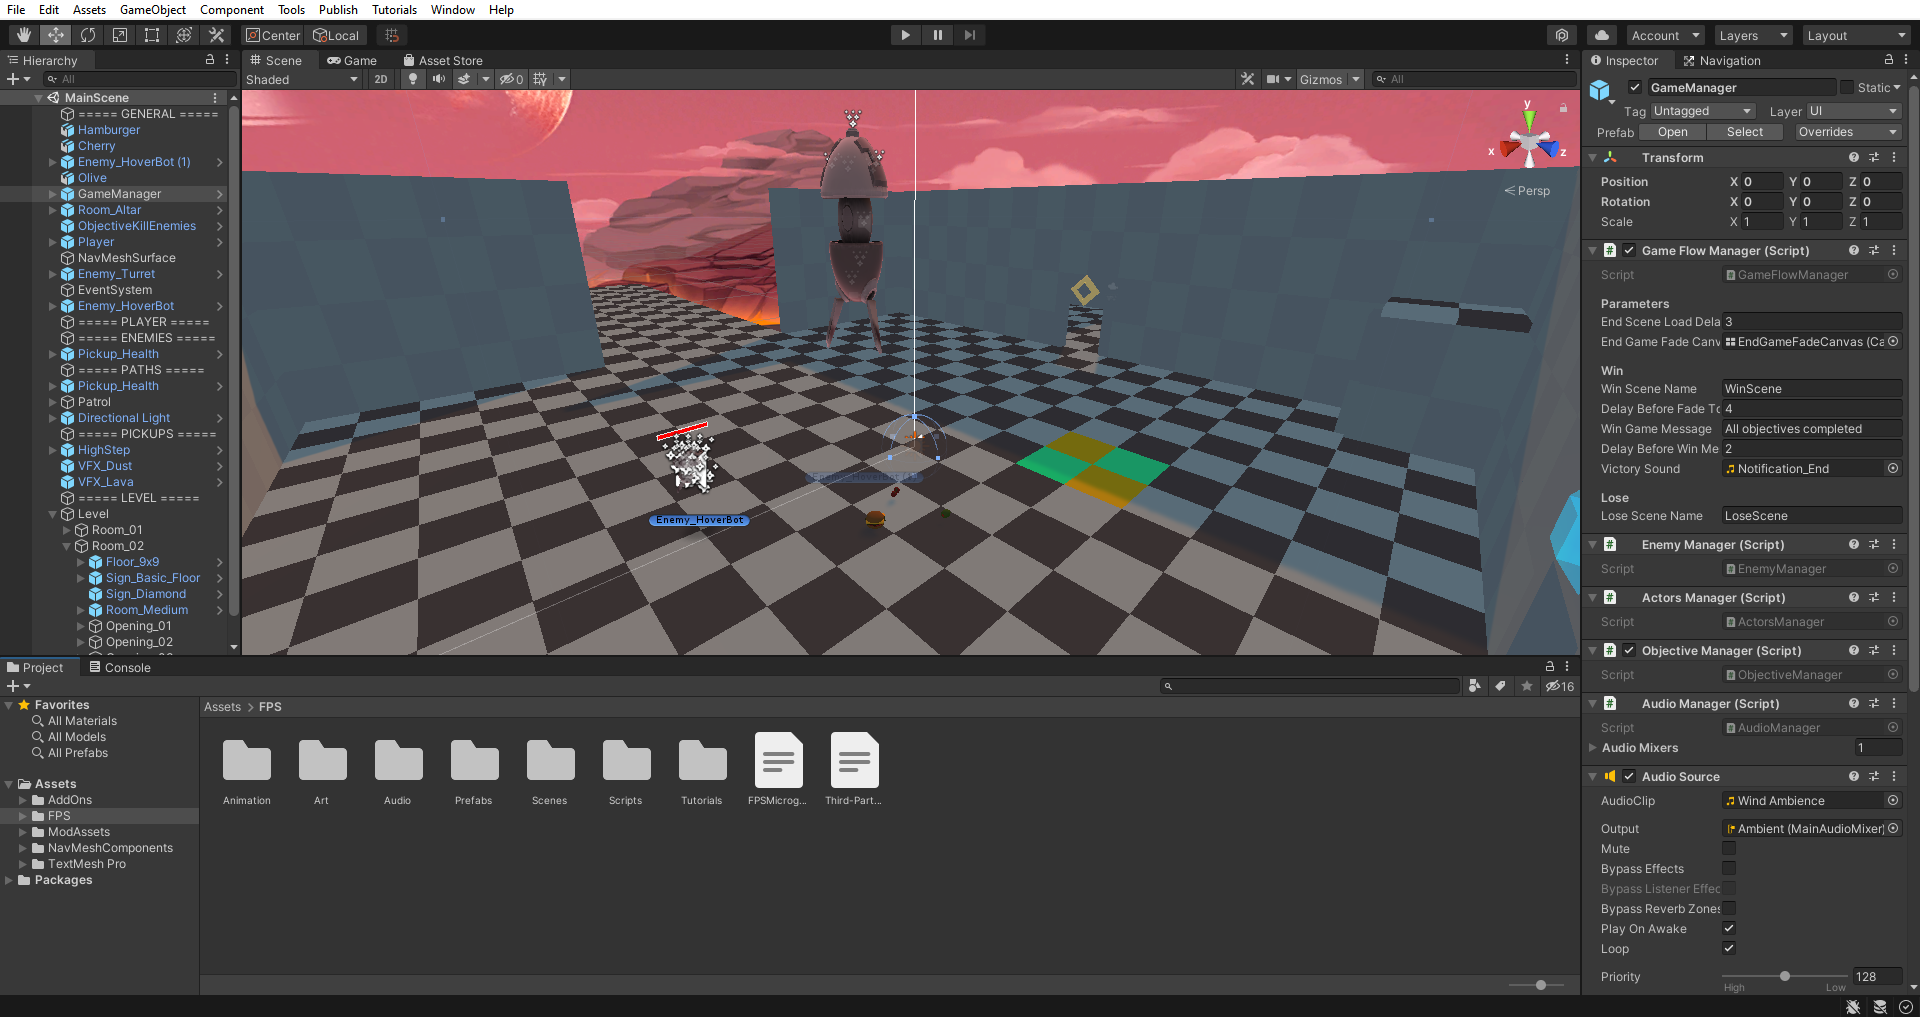
\includegraphics[width=\linewidth]{images/unity_editor.png}
  \caption{Unity Editor}
\end{figure}

The Unity environment is much more extensible than Source. Its package management system makes it easy to obtain first and third-party extensions to the Unity Editor. This same mechanism can also be used to import third-party assets from the internet. In general, using assets is easier compared to Source since Unity supports standard formats, and can even automatically convert formats in some cases.

For scripting, Unity Editor allows scripts to be edited with virtually any text editor. It also natively supports deeper integration with several IDEs: Visual Studio, Visual Studio Code, and JetBrains Rider.

\subsection{Programming}
\subsubsection{Source}
The engine itself is written in C++ so naturally, programming a game with the Source engine is also done in C++. The full source code of the engine can be licensed. Valve also offers a portion of the engine's C++ code with the Source SDK. This is enough to make a game with the SDK, but it doesn't give access to the engine's internals such as its core networking code. The Source engine also comes with it's own Standard Template Library named \texttt{CUtl}, which is located within the \texttt{Tier1} library of the engine.

The engine also supports external scripts using the VScript virtual machine and API. Depending on the version of the SDK, different languages are supported. VScript first shipped with support for the Squirrel language. However, Source Filmmaker uses Python and Portal 2 has limited Lua support.

\begin{figure}[!htp]
  \begin{minted}[
    linenos,
    autogobble=true,
    fontsize=\fontsize{10}{10},
  ]{js}
    function GiveGun(weapon, playerarray) {
      local equipper = Entities.CreateByClassname("game_player_equip")
      equipper.__KeyValueFromInt("spawnflags", 5)
      equipper.__KeyValueFromInt(weapon, 0)
      equipper.ValidateScriptScope()

      for (player in playerarray) {
        EntFireByHandle(equipper, "Use", "", 0, player, null)
      }

      EntFireByHandle(equipper, "Kill", "", 0.1, null, null)
    }
  \end{minted}
  \caption{VScript in Squirrel for CS:GO which equips players}
  \label{fig:source_vscript}
\end{figure}

It is technically possible to add support for scripting with any language, without relying on VScript. Garry's mod did this with Lua, and there is also a project by modders which added Python support.

\paragraph{I/O Entities}
Besides directly programming in C++ and VScript, there is an I/O system by which entities communicate between each other. This system can be leveraged to program entities in Hammer. Effectively, an entity's event can be hooked so that an action is performed on another entity when the event occurs. In fact, entities in Hammer can also be used to run VScripts.

For example, \cref{fig:source_entities} shows some of the entities used to control an elevator. The four stacked \texttt{logic\_relay}s control the doors for each of the four floors. The \texttt{logic\_compare} chooses the next path node for the elevator to travel to. The \texttt{logic\_relay} at the bottom right performs actions when the elevator needs to stop.

\begin{figure}[!htp]
  \centering
  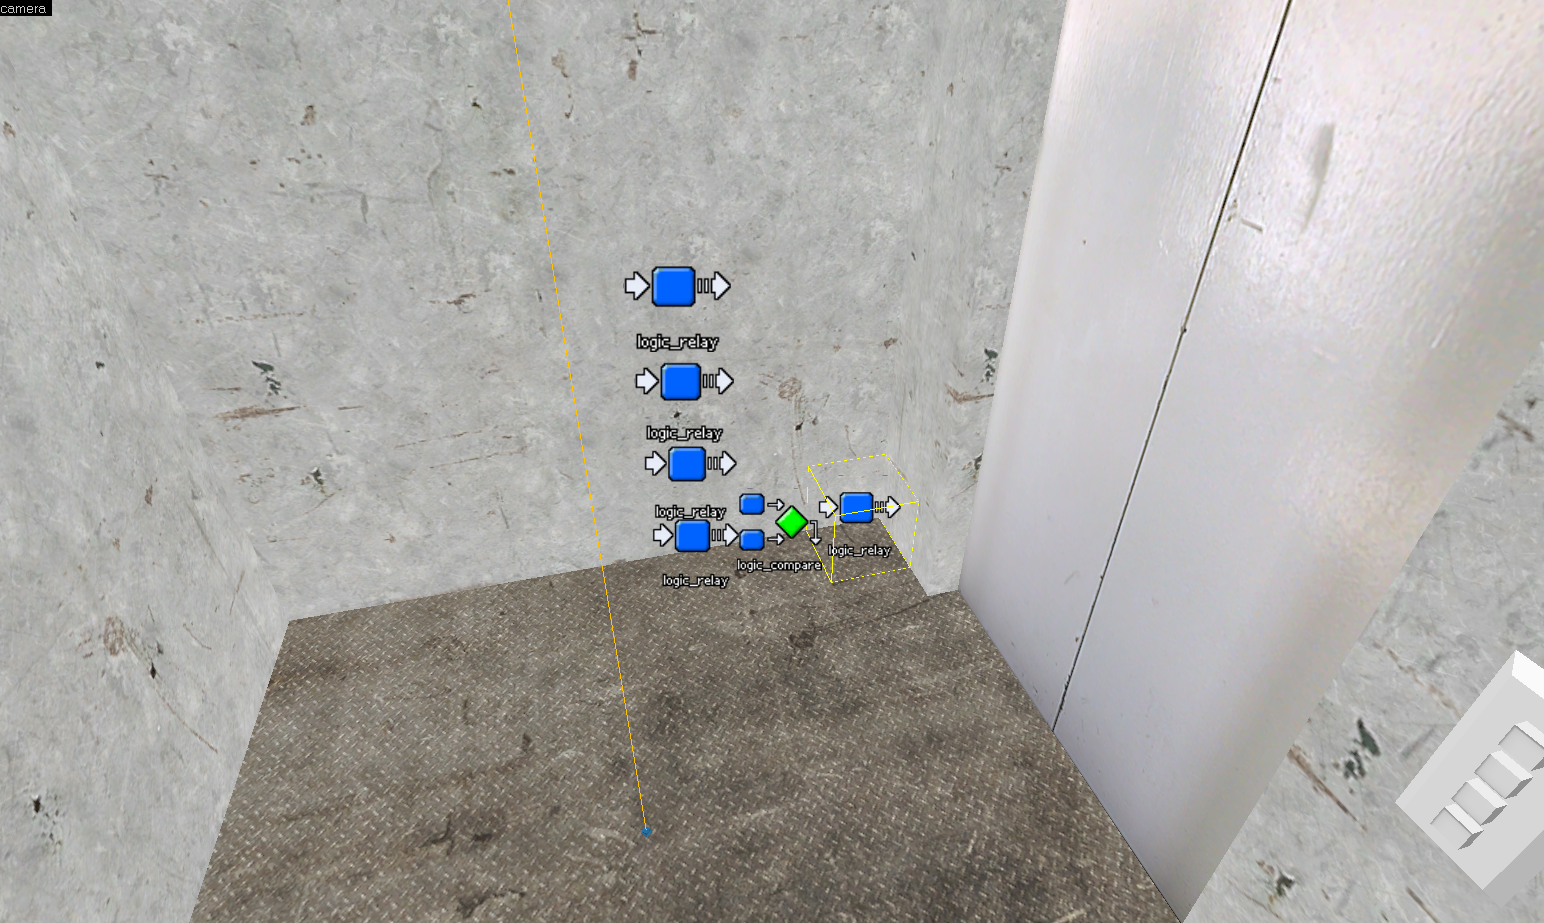
\includegraphics[width=0.75\linewidth]{images/source_io_entities.png}
  \caption{Logic entities for controlling an elevator}
  \label{fig:source_entities}
\end{figure}

The last \texttt{logic\_relay} is pictured in more detail in \cref{fig:source_elev_stop}. The purpose of a \texttt{logic\_relay} is to forward messages; it can turn one input into many outputs. Another entity can trigger the relay, which causes the relay to fire an \texttt{OnTrigger} event. \texttt{elev\_stop} is being triggered by the aforementioned \texttt{logic\_compare}. \texttt{elev\_stop} has four outputs that occur when the \texttt{OnTrigger} event is fired. Each output targets a different entity and sends it some input. The first stops the elevator, the second plays a bell sound, and the last two open doors.

\begin{figure}[!htp]
  \centering
  \subfloat[\centering inputs]{
    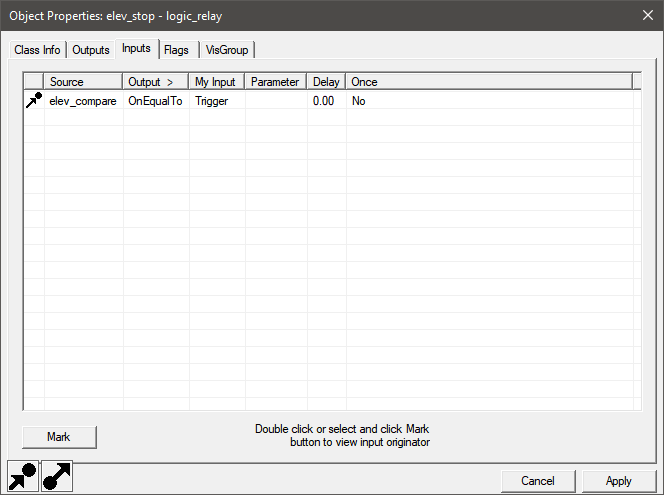
\includegraphics[width=0.45\linewidth]{images/source_io_elev_stop_in.png}
  }
  \qquad
  \subfloat[\centering outputs]{
    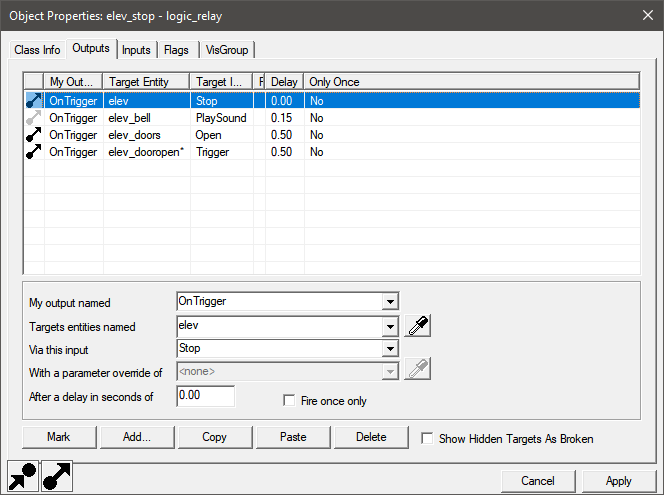
\includegraphics[width=0.45\linewidth]{images/source_io_elev_stop_out.png}
  }
  \caption{The configured I/O of the \texttt{logic\_relay} entity named \texttt{elev\_stop}}
  \label{fig:source_elev_stop}
\end{figure}

\paragraph{Events}
There are many other events, such as one for the player getting hurt or a team winning a round. Data can be associated with an event, for example, which player got hurt or which team won. The \texttt{logic\_eventlistener} entity can be used to listen to events. In C++, \texttt{CGameEventListener::ListenForGameEvent} can be used. The \texttt{CGameEventManager} class can be used to interact with events, be it creating a new event, firing an event, or registering an event listener. Events are declared in various \texttt{.res} files in the \textit{resources} directory of the game. These get loaded using \texttt{CGameEventManager::LoadEventsFromFile}.

\begin{figure}[!htp]
  \begin{minted}[
    linenos,
    autogobble=true,
    fontsize=\fontsize{10}{10},
  ]{js}
    "game_end"              // a game ended
    {
      "winner"  "byte"      // winner team/user id
    }

    "round_start"
    {
      "timelimit" "long"    // round time limit in seconds
      "fraglimit" "long"    // frag limit in seconds
      "objective" "string"  // round objective
    }
  \end{minted}
  \caption{A portion of CS:GO's \textit{resource/gameevents.res}}
  \label{fig:source_gameevents}
\end{figure}

\end{document}
